\documentclass[../main.tex]{subfiles}

\begin{document}
    \chapter{Approach}

    \section{Grad-CAM}
    Gradient-weighted Class Activation Mapping \cite{gradcam}. Technique for producing visual explanations
    about why a Convolutional Neural Network opted for a certain class. The technique is applicable to a wide
    variety of tasks, ranging from image captioning to visual question answering to reinforcement learning, and
    also to a wide variety of CNN architectures. In the context of this work, we'll use this technique to
    produce visuals for an object classification task.
    This technique was designed as a visualization tool to better understand how CNNs reason and to improve
    their interpretability, which is a fundamental property to have for AI systems that wants to be deployed
    in the real world.
    We extracted the Grad-CAM visualization from the last convolutional layer because, as also the authors
    or the technique note, the last conv. layer is the best compromise between high-level semantics and spatial
    localization. The former is a general property of deep learning models: the further the layer from the input,
    the more high-level and meaningful features one can expect to be extracted. The latter is a property of
    Convolutional Feature Maps, which are designed to retain as much spatial information as possible about
    the data.
    The high-level architecture of the method can be seen in the following figure.

	\begin{figure}[h!]
    	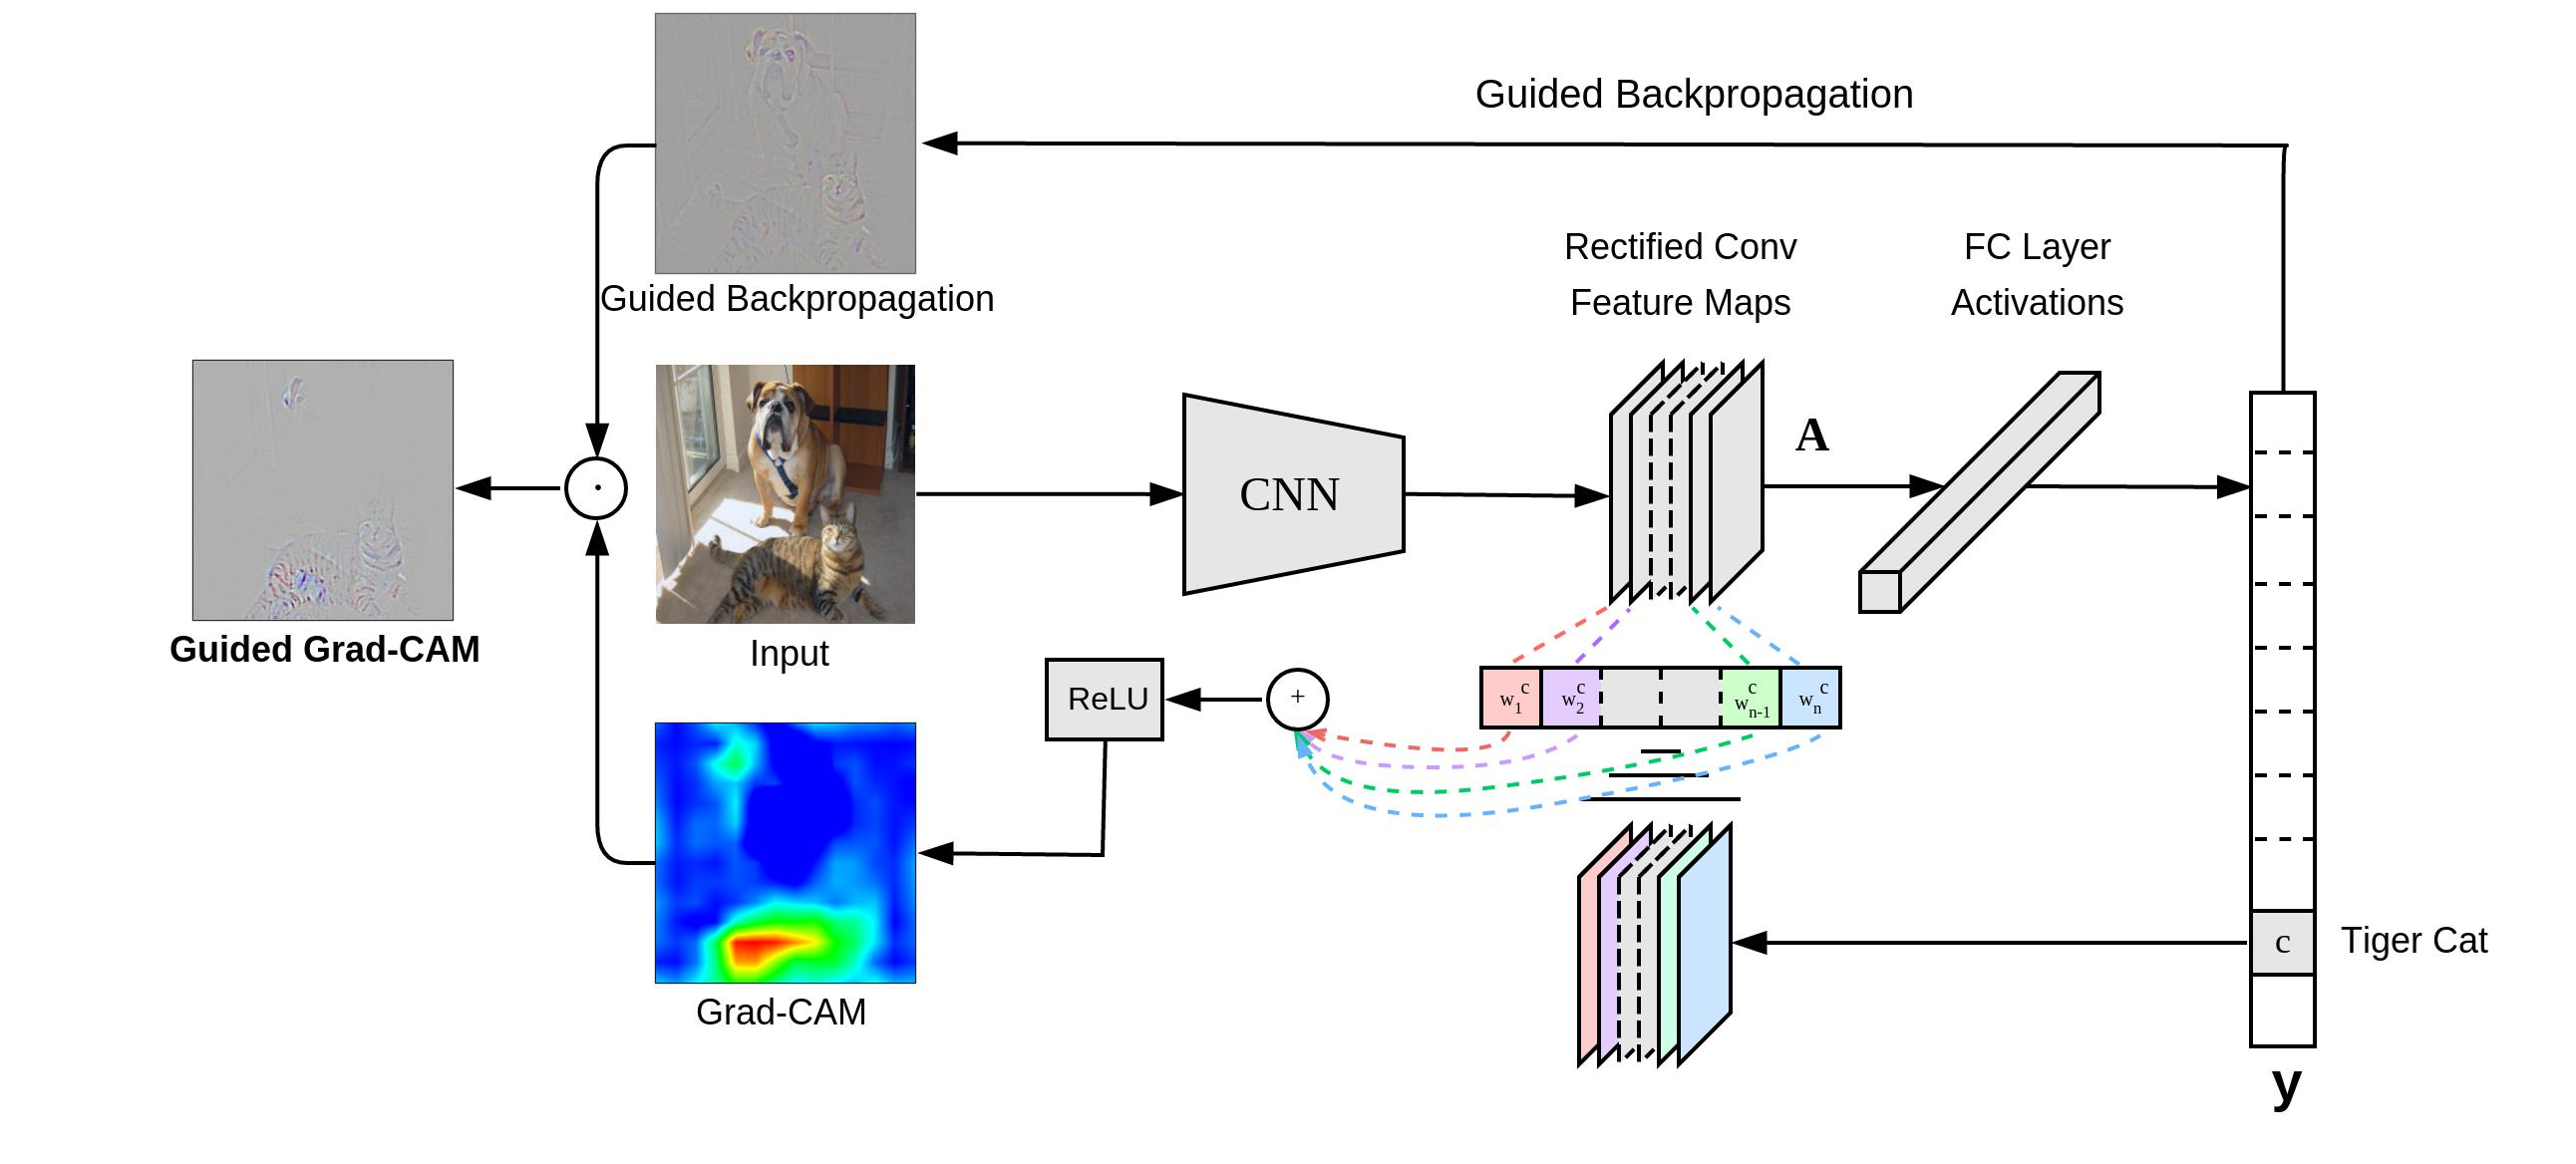
\includegraphics[width=\linewidth]{img/gradcam-architecture.png}
	    \caption{Grad-CAM Architecture, taken from \cite{gradcam}}
    	\label{fig:gradcam-architecture}
	\end{figure}

    Basically, the input image is forward propagated through the network in order to compute the softmax scores
    of the last layer, which we call $y^{c} = f(x)$, where $f()$ is the input-output network mapping.
    If we were training the network, at this point we would have computed the gradients of the
    last layer neurons with respect to some loss function, like cross-entropy. Instead, in Grad-CAM, we manually
    create these gradients. In particular, we set them to one for the neuron corresponding to the class of interest,
    while all the other neurons are set to zero.
    $$ \frac{\partial y^{c}}{\partial \theta_{output}} = [0, 0, \ldots 1, 0, 0, \ldots] $$
    Then, we backward propagate these gradients through the network untill
    the last convolutional layer, where the Grad-CAM map is created. Assume that the last conv. layer feature maps are
    in $ \mathbb{R}^{K \times H \times W} $, where $H$ and $W$ are respectively the height and the width of each feature
    map, and $K$ is the number of feature maps. The map that will be generated is thus in $\mathbb{R}^{H \times W}$.
    The generation procedure has multiple steps:
    \begin{enumerate}
        \item Compute the weight of each feature maps. We want a number measuring how much each filter contributed to
            the final score. It is therefore natural to compute this number as the derivative of the output gradients
            with respect to the weights of the filter. These derivatives are then global average pooled in order to get
            a single number:
            \begin{equation}
                w_{k}^{c} = \frac{1}{Z} \sum_{i = 1}^{h} \sum_{j = 1}^{w} \frac{\partial y^{c}}{\partial F_{i, j}^{k}}
            \end{equation}
            $w_{k}^{c}$ is the weight of feature map $k$ with respect to target class $c$, while $F$ is the feature map
            itself. We can see that the derivative is positive if an increase of the value of the pixel $F_{i, j}^{k}$ yields
            an increase of the value of $y^{c}$.
        \item The Grad-CAM map is obtained by performing a rectified weighted linear combination of the forward feature maps:
            \begin{equation}
                M^{c} = ReLU \left( \sum_{k = 1}^{K} w_{k}^{c} F^{k} \right)
            \end{equation}
    \end{enumerate}
    The $ReLU()$ function simply set to zero all the negative values. The Grad-CAM technique uses this function to retain only
    the values that have a \textit{positive} influence on the class decision.
    Once the Grad-CAM map is generate, it is then upsampled to the pixel space using bi-linear interpolation, then a heatmap
    is generated from the values and the heatmap is point-wise multiplied with the output of the Guided-BackPropagation procedure
	\cite{guidedbackprop}, to produce the final result Guided-GradCAM.

    \subsection{Grad-CAM for domain localization}

    \section{Spatial Pyramid Pooling}
    Convolutional Networks can be thought of as composed by two parts, a feature extractor and a classifier. The former is composed
    by convolutional layers, while the latter by fully-connected layers, that is simply an affine mapping followed by some non-linearity.
    Each convolutional layer has three sequential stages: a convolution operation, a pooling operation, and a non-linearity operation.
    The pooling operation is needed to reduce the dimensionality of the data and to improve robustness with respect to input distortion.
    Usually, Max Pooling is used. Max pooling is a sliding window in which for each window, the pixel with the max value is taken as output.
    Spatial Pyramid Pooling is a method that was used extensively in computer vision algorithms before the deep learning revolution.
    This paper \cite{sppooling} introduced the technique in the context of deep networks. Basically, a Spatial Pyramid Pooling operation
    it's nothing but multiple Max Pooling ops performed at different window sizes and then concatenated together. This seemingly simple
    alteration of the standard pooling layer has profound implications, such that:
    \begin{itemize}
        \item CNNs with standard Max Pooling layers must take in input images of fixed size (say $224 \times 224$). With SPP instead, the network can take in input images of arbitrary sizes, scales and aspect ratios.
        \item The network is much more robust to distortions and alterations of the input, because the pooling is done at multiple levels.
        \item Classification accuracy is increased.
    \end{itemize}


    \section{Domain-Multiplicative Fusion}
    \subsection{Architecture Design}
\end{document}
